\section{Experimental evaluation}\label{sec:eval}
This section provides results of our experiments and a discussion of relevant findings. We begin by establishing baseline performance for our Zookeeper testbed which support reasoning for follow-up experiments with synchronization primitves. The synchronization mechanisms benchmarked are Queues and Locks, each implemented with both, synchronous and asynchronous messaging. For this quantitative analysis we focus on average latency and graceful degradation.

%\subsection{Experimental setup}
%The testbed consists of 5 machine containing a quad-core Xeon 2135, 16GB RAM and commodity 500GB 7.2k rpm disks running stock Ubuntu 12.04. They are interconnected with 1Gbps Ethernet on a single switch. A separate machine acts as client without being a Zookeeper server. For our experiments these nodes for quorums out of 1, 3 or 5 nodes as indicated. The server-side uses Zookeeper version 3.3.5 whereas the client-side implementation of benchmarks uses Python bindings for the baseline "smoke test" and Java bindings for Locks and Queues.
%In order the measure the impact of client-server and server-server latency we control the transmission latency of packets transmitted between nodes using the Linux "Traffic Control" utility. We automate the process of enumerating client-server and server-server latency pairs and repeatedly run the experiments and average the results to reduce the impact of jitter.

%\note{Average RTT for pings is (ping lat)
%Average network throughput is (throughput=). this for inter-cluster and cluster to hamilton.}

%\begin{figure}[h]
%\centering
%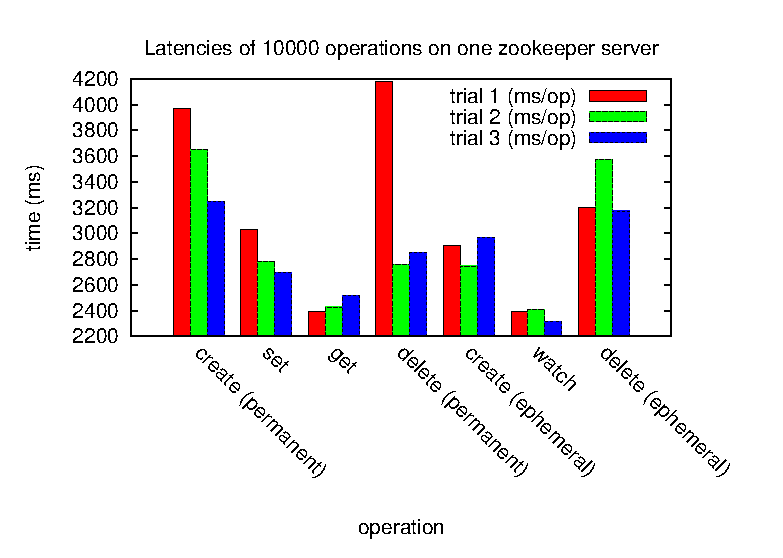
\includegraphics[scale=0.75]{img/1_machine_1_server.eps}
%\caption{}
%\label{fig:1machine_1server_latency}
%\end{figure}

\subsection{Baseline performance}
%In this section we will perform experiments to establish a baseline for later experiments using the Zookeeper smoke test package. We would like to establish limits on the system. These limits represent workloads and environment conditions that will saturate the system. Workload is represented by the number of requests per second and the type of requests. Environment conditions are the number of zookeeper servers and condition of links connecting them.

%We begin by measuring the latencies of basic Zookeeper operations. Our first experiment is performed on one machine holding a single zookeeper instance and the client. This means that there is no network communication overhead for consensus. One client issues 10000 calls of each tested operations and we report the total time required to complete them. The results as shown in Figure~\ref{fig:1machine_1server_latency}\footnote{These results are obtained from a different server than those in next figures. It will be changed in the final draft for consistency} for asynchronous versions of operations. We report detailed results of three trials to show the variability of zookeeper behavior. In the figure we report latencies of adding and deleting in both cases, permanent and ephemeral. Creating a permanent node incur more bandwidth than creating a ephemeral node. On the other hand, deleting an ephemeral node incur more bandwidth than deleting permanent nodes (except for first trial that is due variability of behavior). Other observations are that set operations are more expensive than get operations, as expected. Also, the implementation of watches is efficient.

%\begin{figure}[h]
%\centering
%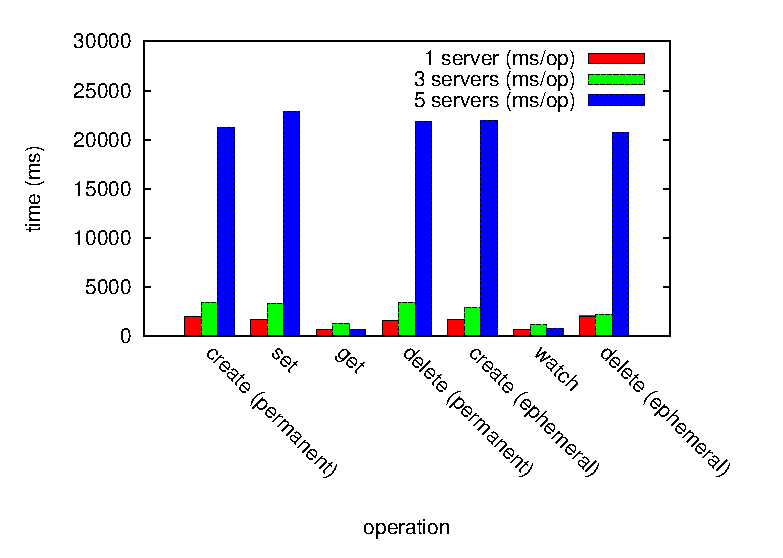
\includegraphics[scale=0.75]{img/1_machine_diff_cpu.eps}
%\caption{Latencies of 10000 operations on various number of zookeeper servers with asynchronous operations on one machines}
%\label{fig:1machine_diffcpu_latency}
%\end{figure}

%\begin{figure}[h]
%\centering
%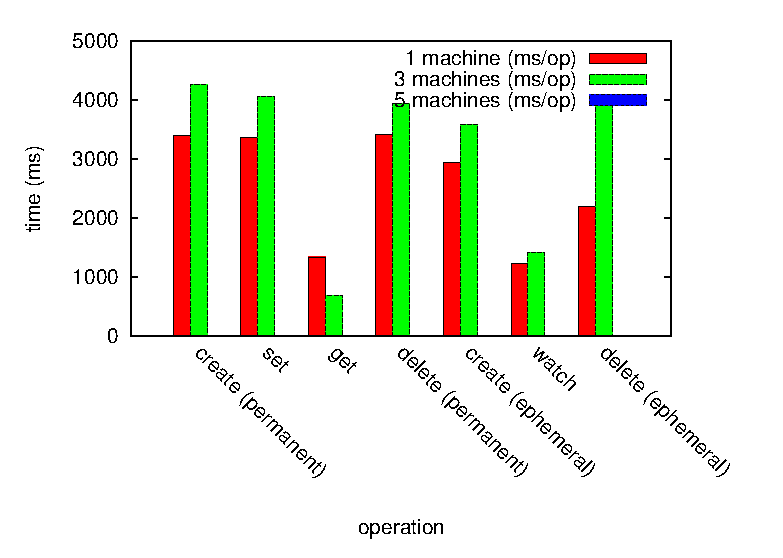
\includegraphics[scale=0.75]{img/1_machine_diff_machines.eps}
%\caption{Latencies of 10000 operations on three zookeeper server with asynchronous operations while changing number of machines}
%\label{fig:1machine_diffservers}
%\end{figure}

%Our next set of results are done to test the effect of increasing the number of Zookeeper servers. Results are shown in Figure~\ref{fig:1machine_diffcpu_latency}. These results are collected when running all servers in one machine. Thus, communication overhead between servers is minimal. As shown in the figure, increasing the number of servers to five servers have a dramatic effect on latency.
%In Figure~\ref{fig:1machine_diffservers} we show results of fanning out Zookeeper servers. We test the performance of three Zookeeper servers running on different number of machines, namely 1, 2, and 3 servers\footnote{results for five servers are not ready yet}. \ldots

\begin{figure}[h]
\centering
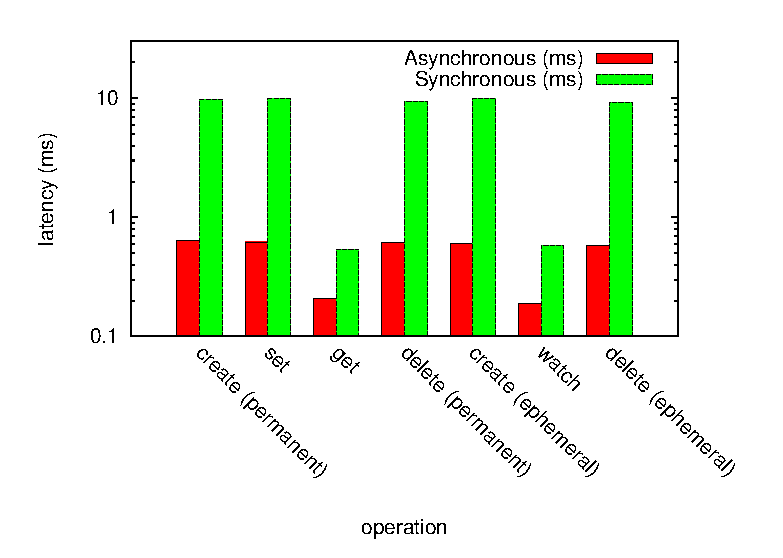
\includegraphics[scale=0.75]{img/ops_latencies_logscale.eps}
\caption{Zookeeper basic operations latencies for a cluster of five servers}
\label{fig:ops_latencies}
\end{figure}

Our first experiments test basic Zookeeper operations' latencies. We test both synchronous and asynchronous versions of these operations. For testing we use zk-smoketest\footnote{https://github.com/phunt/zk-smoketest}. Each operation is run for a thousand time and we report average latency. Results are shown in Figure~\ref{fig:ops_latencies}. Synchronous operations block until the operation is performed, thus giving an indication on the total time taken to perform the actual operation. Asynchronous operations on the other hand do not block. The figure shown that synchronous operations takes more than ten times the latency of asynchronous operations for \emph{put} operations (operations that update znodes), and around double the latency for \emph{get} operations (operations that does not update znodes). Another interesting observation is that for both synchronous and asynchronous operations set operations (and get operations) have a close latency. This will enable us to pick only a representative of those operations to collect more thorough results. In the next experiment we use create as a representative for set operations. We chose create as it is involved in all our synchronization primitives.

\begin{figure}[h]
\centering
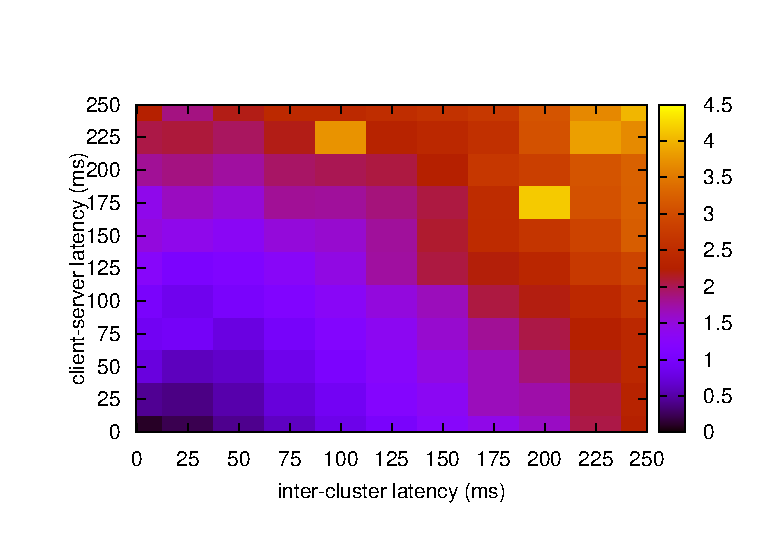
\includegraphics[scale=0.75]{img/async_ops_latencies_heatmap.eps}
\caption{Zookeeper asynchronous average create operation latency with different inter-cluster and user-server RTTs}
\label{fig:async_heatmap}
\end{figure}

\begin{figure}[h]
\centering
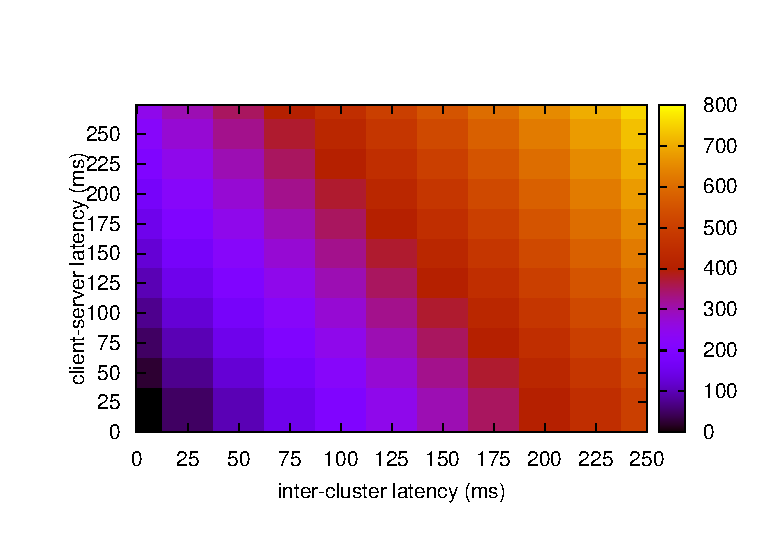
\includegraphics[scale=0.75]{img/sync_ops_latencies_heatmap.eps}
\caption{Zookeeper synchronous average create operation latency with different inter-cluster and user-server RTTs}
\label{fig:sync_heatmap}
\end{figure}

We would like to test the effect of latency on Zookeeper operations. Therefore, we introduce latency in two ways. First, we vary the RTT between the client machine and the cluster and call it \emph{user-to-server} RTT. Second, we vary RTT between Zookeeper servers and we will call it \emph{inter-cluster} RTT. Reported numbers are not the final RTT, but the addition to the original RTT. Since the original RTT is very low compared to our introduced values, reported values act as a good approximation. The first set of results are of asynchronous create operation while varying user-to-server and inter-cluster RTTs and is shown in Figure~\ref{fig:async_heatmap}. Asynchronous creates average values do not exceed 4.5ms in our experiment, although RTTs go up to 250. This is because asynchronous operations are allowed to start immediately after invokation of the previous operation. Thus, these results act as an indicator of the level of parallelism that can be supported by Zookeeper. Assuming worst case, we can calculate a lower bound on the average number of concurrent asynchronous creates by dividing RTT by maximum reported latency, hence $\frac{250}{4.5} = 55.56$ operations. An interesting finding is that though asynchronous requests are used, both user-to-server and inter-cluster RTTs have an effect on operation latency.

Now we test synchronous create while varying user-to-server and inter-cluster latencies. Results are shown in Figure~\ref{fig:sync_heatmap}. Since synchronous creates are used, reported results are the sum of user-to-server RTT and time it takes for Zookeeper servers to process the operation. From the linear relation observed with user-to-server latency, it is apparent that two RTTs are involved in the exchange. Those RTTs corresponds to starting the connection and issuing the create operation. Another observation is that at least one (inter-cluster) RTT is involved in the cluster-side processing of the operation. However, as the inter-cluster RTT increase the latency increase faster than the rate of RTT change. 

\begin{figure*}[ht!]
     \begin{center}
        \subfloat[Latency of synchronous queue locks]{
            \label{fig:first}
            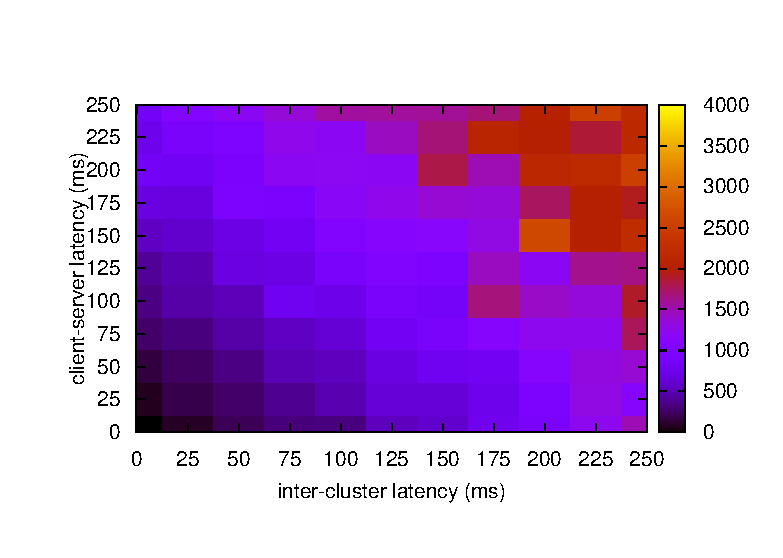
\includegraphics[width=0.5\textwidth]{img/primitives_latencies_varDelay_syncqueue.eps}
        }
        \subfloat[Latency of synchronous TAS]{
           \label{fig:second}
           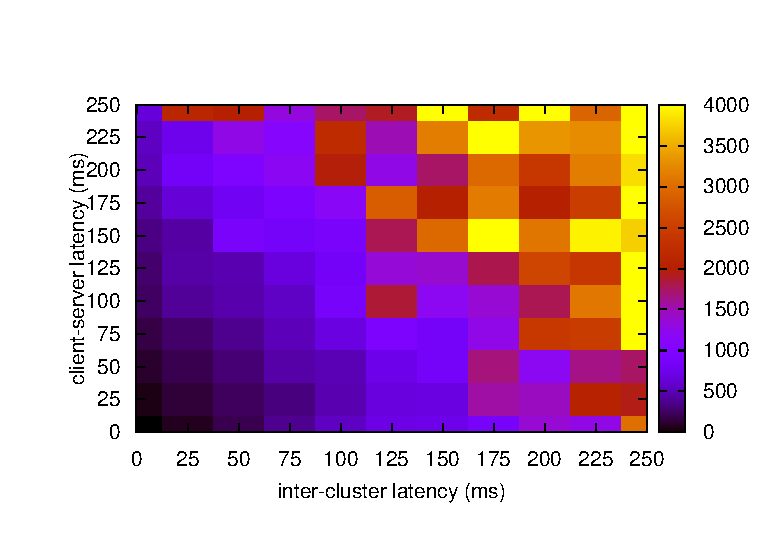
\includegraphics[width=0.5\textwidth]{img/primitives_latencies_varDelay_syncTAS.eps}
        }\\ %  ------- End of the first row ----------------------%
        \subfloat[Latency of asynchronous queue locks]{
            \label{fig:third}
            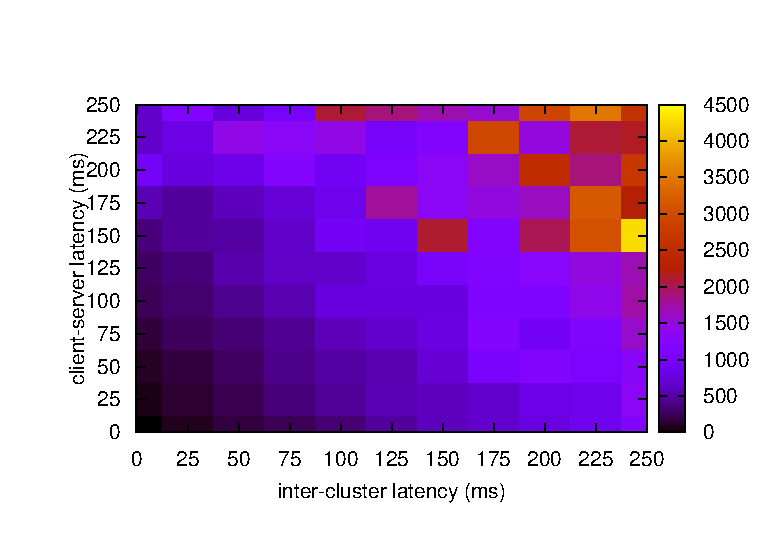
\includegraphics[width=0.5\textwidth]{img/primitives_latencies_varDelay_asyncqueue.eps}
        }
        \subfloat[Latency of asynchronous TAS]{
            \label{fig:fourth}
            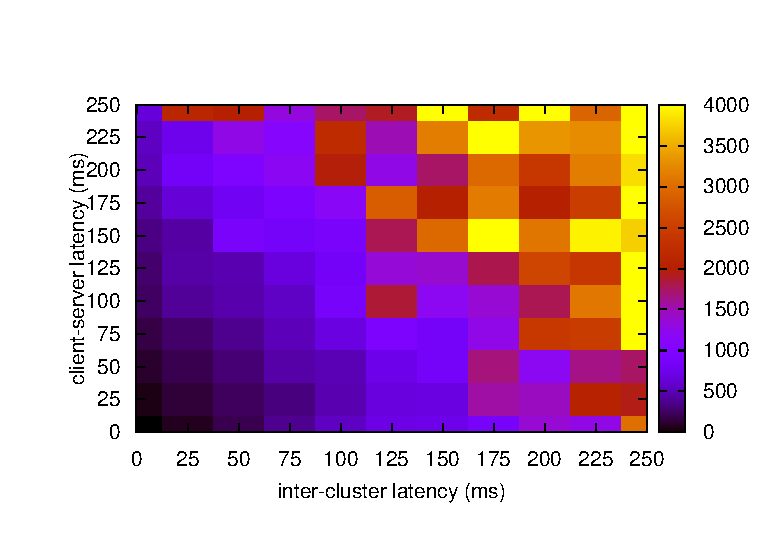
\includegraphics[width=0.5\textwidth]{img/primitives_latencies_varDelay_asyncTAS.eps}
        }
    \end{center}
    \caption{
        Heatmaps of different synchronization primitives' latencies while varying inter-cluster RTT and user-to-server RTT.
     }
   \label{fig:subfigures}
\end{figure*}

\begin{figure}[h]
\centering
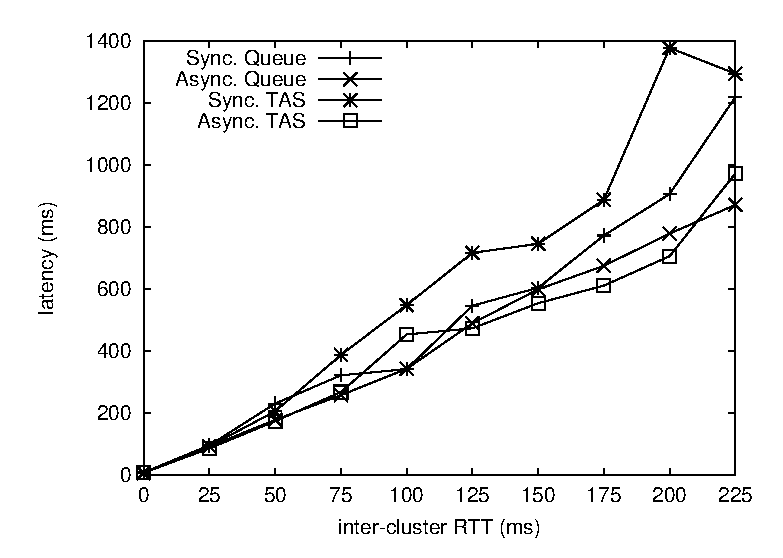
\includegraphics[scale=0.68]{img/primitives_fixUserLatency-0.eps}
\caption{Synchronization primitives latency while varying inter-cluster latency and not changing user-to-server latency}
\label{fig:primitives_vary_intercluster}
\end{figure}

\begin{figure}[h]
\centering
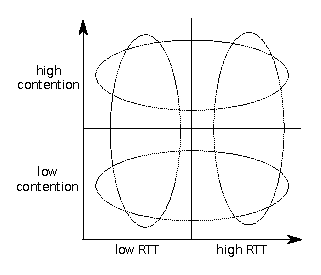
\includegraphics[scale=1.55]{img/spectrum.eps}
\caption{The spectrum of RTT and contention used for our experiments. Ovals represent a span of a performed experiment}
\label{fig:spectrum}
\end{figure}

\begin{figure}[h]
\centering
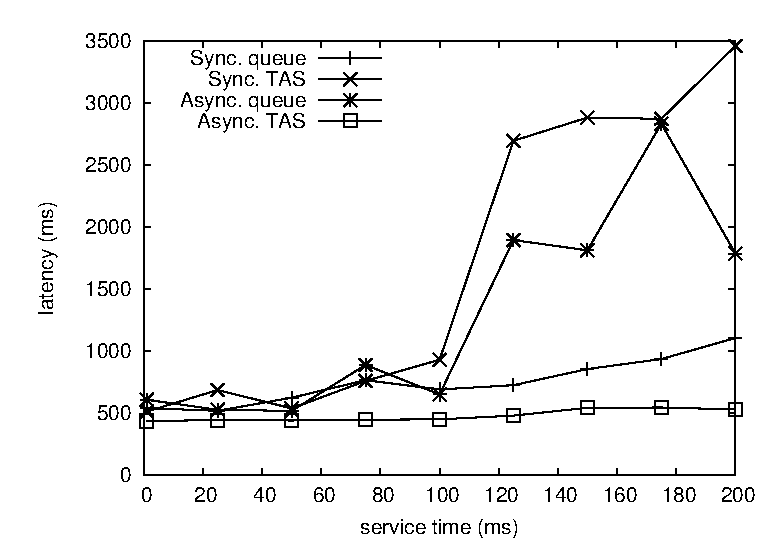
\includegraphics[scale=0.68]{img/primitives_vary-contention_rtt-100.eps}
\caption{Synchronization primitives latency while varying contention and fixing RTT to 100ms (varying contention with high RTT)}
\label{fig:primitives_vary_contention_rtt100}
\end{figure}

\begin{figure}[h]
\centering
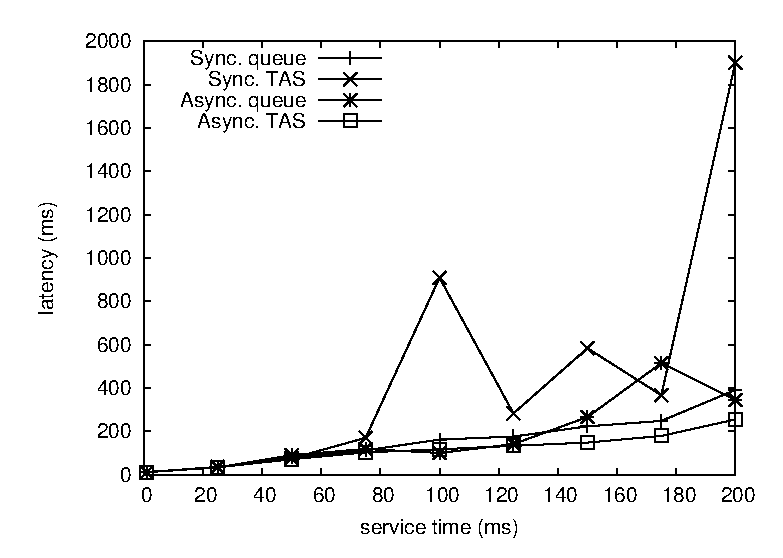
\includegraphics[scale=0.68]{img/primitives_vary-contention_rtt-0.eps}
\caption{Synchronization primitives latency while varying contention and no additional delay to RTT (varying contention with low RTT)}
\label{fig:primitives_vary_contention_rtt0}
\end{figure}

\begin{figure}[h]
\centering
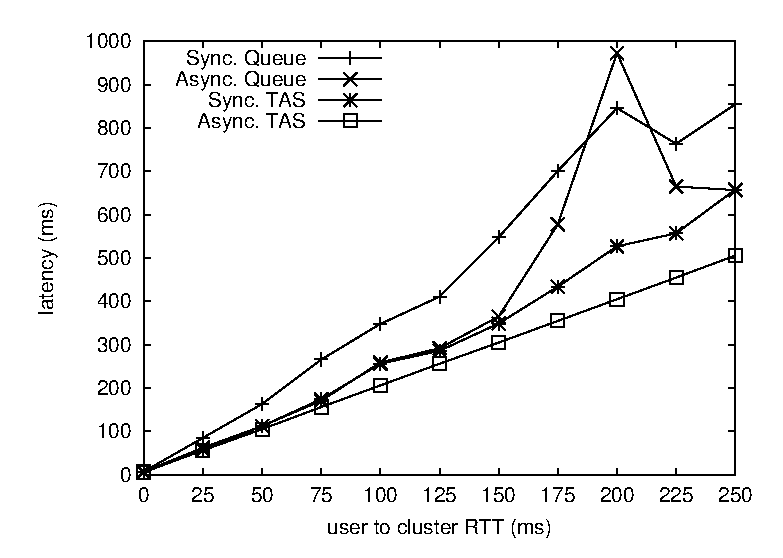
\includegraphics[scale=0.68]{img/primitives_fixClusterLatency-0.eps}
\caption{Synchronization primitives latency while varying user-cluster RTT, with no additional inter-cluster delay, and fixing service time to 1ms and interarrival time to 500ms (low contention with varying latency)}
\label{fig:primitives_vary_delay_lowcontention}
\end{figure}

\begin{figure}[h]
\centering
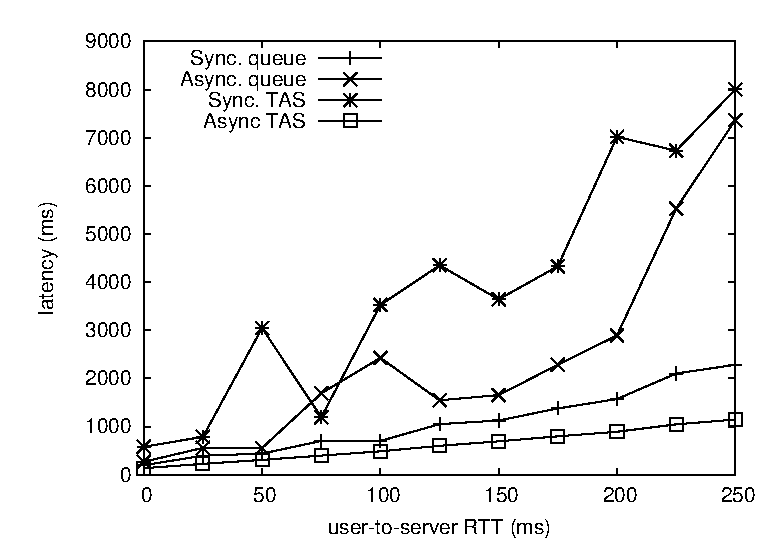
\includegraphics[scale=0.68]{img/fixService-150_varyLatency.eps}
\caption{Synchronization primitives latency while varying user-cluster RTT, with no additional inter-cluster delay, and fixing service time to 150ms and interarrival time to 200ms (high contention with varying latency)}
\label{fig:primitives_vary_delay_highcontention}
\end{figure}

\subsection{synchronization primitives}
%The experiments in this section focus on two fundamental synchonization primites, locks and queues, which are commonly found as builind blocks of larger coordination schemes. The implementation of synchronous primitives follows the Zookeeper recipies with minor improvements, while the asynchronous implementation is described in detail in the following.
%Locks follow a test-and-set approach by repeatedly issuing create requests and upon successful response from the server assuming mutual exclusion. The lock is then released by deleting the node. The synchonous lock issues a single create request for a fixed node path and blocks until a response arrives. On a positive response mutual exclusion is guaranteed. A negative respose is directly followed up by another create request. This lock has at most a single request or response in transit at a given time. The asynchonous lock issues create requests on a timer basis until a positive response is recorded. This implementation has multiple requests and responses in transit at a time and effectively "polls" the availability of the lock. This puts higher load on the network and server, but may reduce the time taken to aquire a lock by avoiding an additional notify-request roundtrip.
%Queues are built using server-side sequentially increasing ids for creating the node. After the node is created the nodes predecessors are obtained and upon their deletion mutual exclusion is guaranteed. As for locks release is performed by deleting the node. The synchonous implementation creates a sub-node, and upon sucess notification requests the list of all siblings from the server using "getChildren". If the created node holds the lowest Id mutual exclusion is guaranteed, otherwise a watch on deletion of its predecessor is installed. The asynchonous queue issues the create request in parallel with polling children at a fixed interval. When the create request returns the obtained Id and the most recent list of children contains the Id in first place mutual exclusion is guaranteed. This approach follows the same trade-offs as asynchonous locks, but can be extended to install a watch on the predecessor and stop polling after a round trip interval.

In this section we will study our primitives while we vary to important metrics. The first metric is traditionally important for synchronization primitives, namely contention. We vary contention by fixing interarrival time of requests to enter the critical section while varying the service time (\emph{e.g.}, time spent inside the critical section). The second metric is latency. Specifically we are interested in large delays that characterize multi-datacenter communication. The goal of this study is to come out with conclusions on which primitives to use giving different contention and network conditions.

We test all our synchronization primitives while we vary user-to-server and inter-cluster RTTs. These experiments will give us hints on how these primitives act with different RTTs, what is the difference between inter-cluster and user-to-server effects, and what primitives are better when large RTTs are experienced. We show these results in Figure~\ref{fig:subfigures}. In them, interarrival time between lock requests is exponentially distributed with a mean of 500ms and time spent in the critical section is exponentially distributed with a mean of 1ms. Asynchronous TAS are the most efficient and stable amongst studied primitives. On the other hand, synchronous TAS perform poorly when RTT is high. Queue implementations are better than synchronous TAS for large delays, though are comparable and slightly worse with low RTTs. We will examine relashionship between primitives in specific cases later in this section. 

In the following we study the two-dimensional spectrum of RTT and contention effect on synchronization primitives' latency. We only vary user-to-server RTT. Inter-cluster latency affect the throughput of all synchronization primitives with the same magnitude. This is because synchronization primitives on top of Zookeeper control the exchange of messages between the user and the server and does not affect the exchange of inter-cluster controls. This is apparent in Figure~\ref{fig:primitives_vary_intercluster}, where we vary inter-cluster latency while fixing user-to-server latency and contention. In the figure it is observed that increasing inter-cluster latency have a fixed additive effect on all primitives. We performed four experiments to examine the possible spectrum of values while varying RTT and contention. The span of each experiment is represented as an oval in Figure~\ref{fig:spectrum}. The following are description of our results:
\begin{itemize}
\item{\emph{High RTT and varied contention}: Figure~\ref{fig:primitives_vary_contention_rtt100} shows the result of the effect of contention with high RTT. We fix user-to-server RTT to 100ms. Interarrival times between lock requests are fixed to 200ms. Until a critical point (100ms service time in this case) all primitives perform similarly. When service time is above 100ms Asyncronous queue and synchronous TAS performs poorly. Thus, for high RTT and high contention synchronous queue is better than synchronous TAS.}
\item{\emph{Low RTT and varied contention}: Figure~\ref{fig:primitives_vary_contention_rtt0} display results for the effect of contention with low RTT. We keep the original user-to-cluster latency as it is (\emph{i.e.}, 0.2ms). Interarrival times between lock requests are fixed to 200ms. Here we notice that the effect is not as visible as the high RTT case. However, all primitives perform closely except for asynchronous queues.}
\item{\emph{Low contention and varied RTT}: this experiments show the effect of varying RTT while having low contention (\emph{i.e.}, service time is 1ms and interarrival of requests is 500ms). Figure~\ref{fig:primitives_vary_delay_lowcontention} shows obtained results. From these results it is shown that for low contention, TAS protocols perform better than queue ones. As RTT increases, the different in latency becomes more apparent. Asynchronous TAS is better than synchronous TAS which perform closely to asynchronous queues for low RTT. Thus, we conclude that for low contention, TAS protocols perform better, specially for large RTTs. }
\item{\emph{High contention and varied RTT}: this experiments show the effect of varying RTT while having high contention (\emph{i.e.}, service time is 150ms and interarrival of requests is 200ms). Figure~\ref{fig:primitives_vary_delay_highcontention} shows obtained results. Confirming our results when we tested varying contention, asynchronous TAS and synchronous queues perform best, specially for high contention.}
\end{itemize}

Giving the results of our previous experiments, we are now able to infer the tradeoffs of using synchronization primitives with varying RTT and contention conditions. The following summarizes our findings relative to each part of the RTT and contention spectrum:
\begin{itemize}
\item{\emph{Low RTT/low contention}: }
\item{\emph{Low RTT/high contention}: }
\item{\emph{high RTT/low contention}: }
\item{\emph{high RTT/high contention}: }
\end{itemize}















